\section{Alignment \& belief}

\DndDropCapLine{T}{}here are layers within layers when it comes to the religions found in this world,
however there are \textit{\textbf{pillars that support the foundations of the very structure of reality}}. Each main religion has a \textbf{\textit{unique domain}} tied to it, with divine influence exacted by \textit{few chosen clerics}.

\subsection{Gnocism}
%Lawful Good

The religion governed by the \textit{\textbf{Greater Will}} is known as Gnocism, the \textit{belief in a hidden, uncorrupted supreme being and a flawed \textbf{demiurge}} known as the \textit{\textbf{palm of creation}}, responsible for creating material reality. The \textit{\textbf{main church of Avaticana}} is centred in \textbf{Romulon}, city of the High Elves and serves as the \textit{political and religious hub} for the majority of the known world. The three sub sects of the Church is that of\textbf{ Apophystic Gnocism}, \textbf{Mystic Gnocism }and \textbf{Teleistic Gnocism}. Most folk tend to just serve the church without delving too deep into the theological aspect thereof. Its people are generally peaceful, however ancient \textit{holy wars} were fought quite recently against their greatest rivals the Vhaethiri, believers in \textbf{Aposiopism} and \textit{Her Web of Lies.}

\subsubsection{Religious Leader}
\textbf{The Pontifex, father Indorilius}, \textit{previously a humble Temple Knight}, is the current leader of this religious movement, elected at the \textit{\textbf{Conclave of the Chosen }}for his service in \textit{\textbf{the Crusade of Lies}}.

\subsection{Aposiopism}
%spiders and drow
%Lawful Evil


\subsubsection{Religious Leaders}


\begin{figure}[H]
\centering
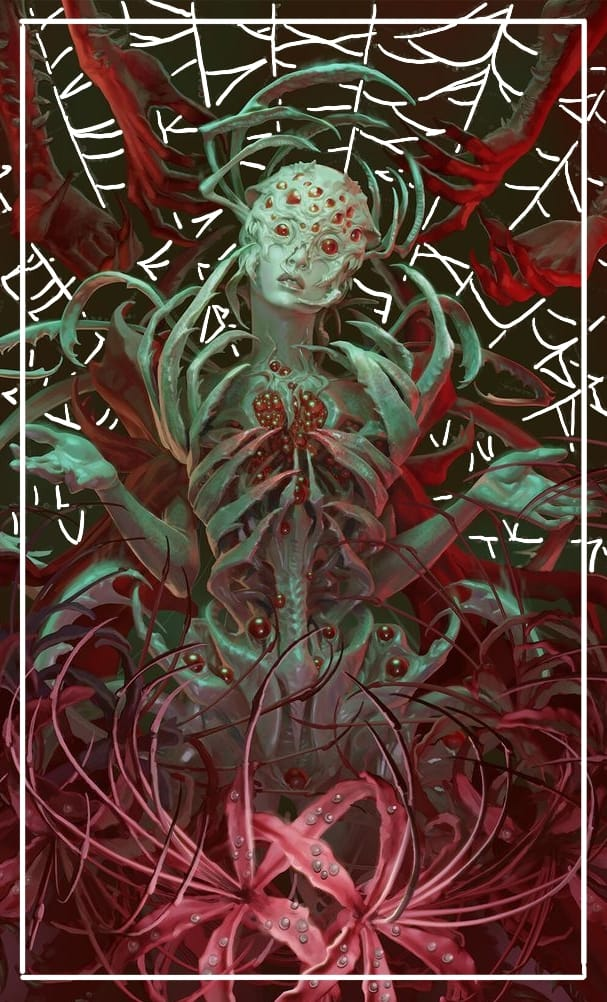
\includegraphics[width=0.22\textwidth]{Images/web.jpeg}
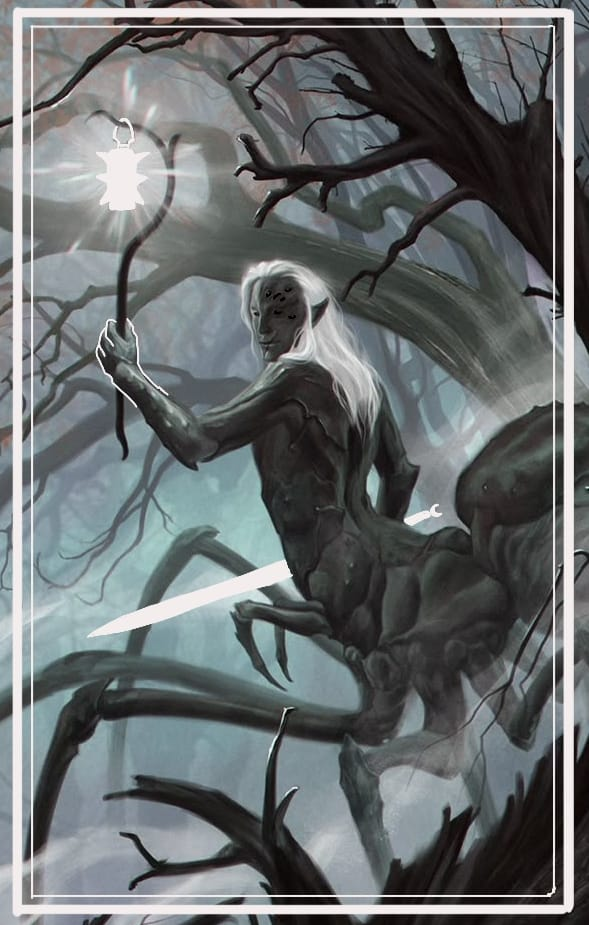
\includegraphics[width=0.232\textwidth]{Images/drider.jpeg}
\end{figure}

\subsection{Tar-Vasham}
%towers and Qunari
%Lawful Neutral

\subsection{Empyrealism}
%frenzied flame
%Chaotic Neutral

\begin{figure}[H]
    \centering
    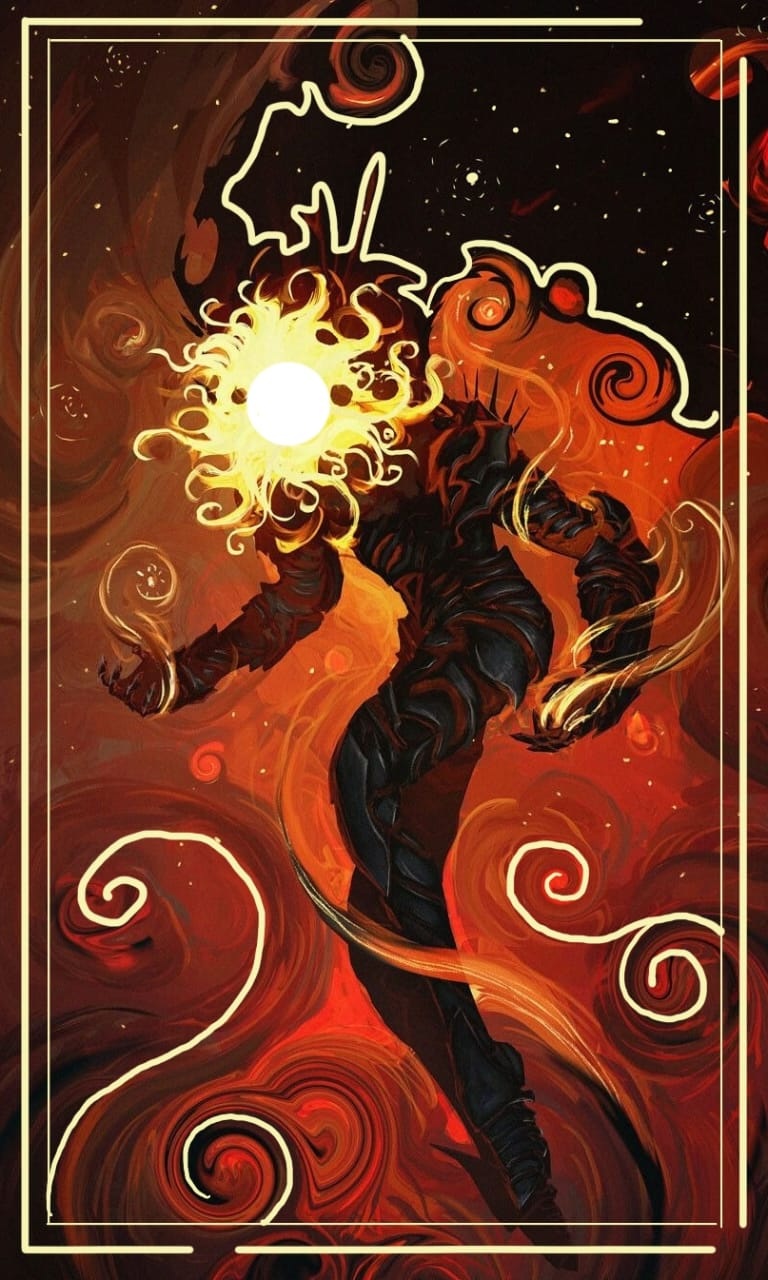
\includegraphics[width=0.71\linewidth]{Images/frenzy_inf.jpeg}
    \label{fig:placeholder}
\end{figure}

\subsection{Viridism}
%verdant oath, wood elves and nature
%Chaotic Good

\subsection{Miasmism} 
%Ruinous Rot
%Chaotic Evil

\begin{figure}[H]
    \centering
    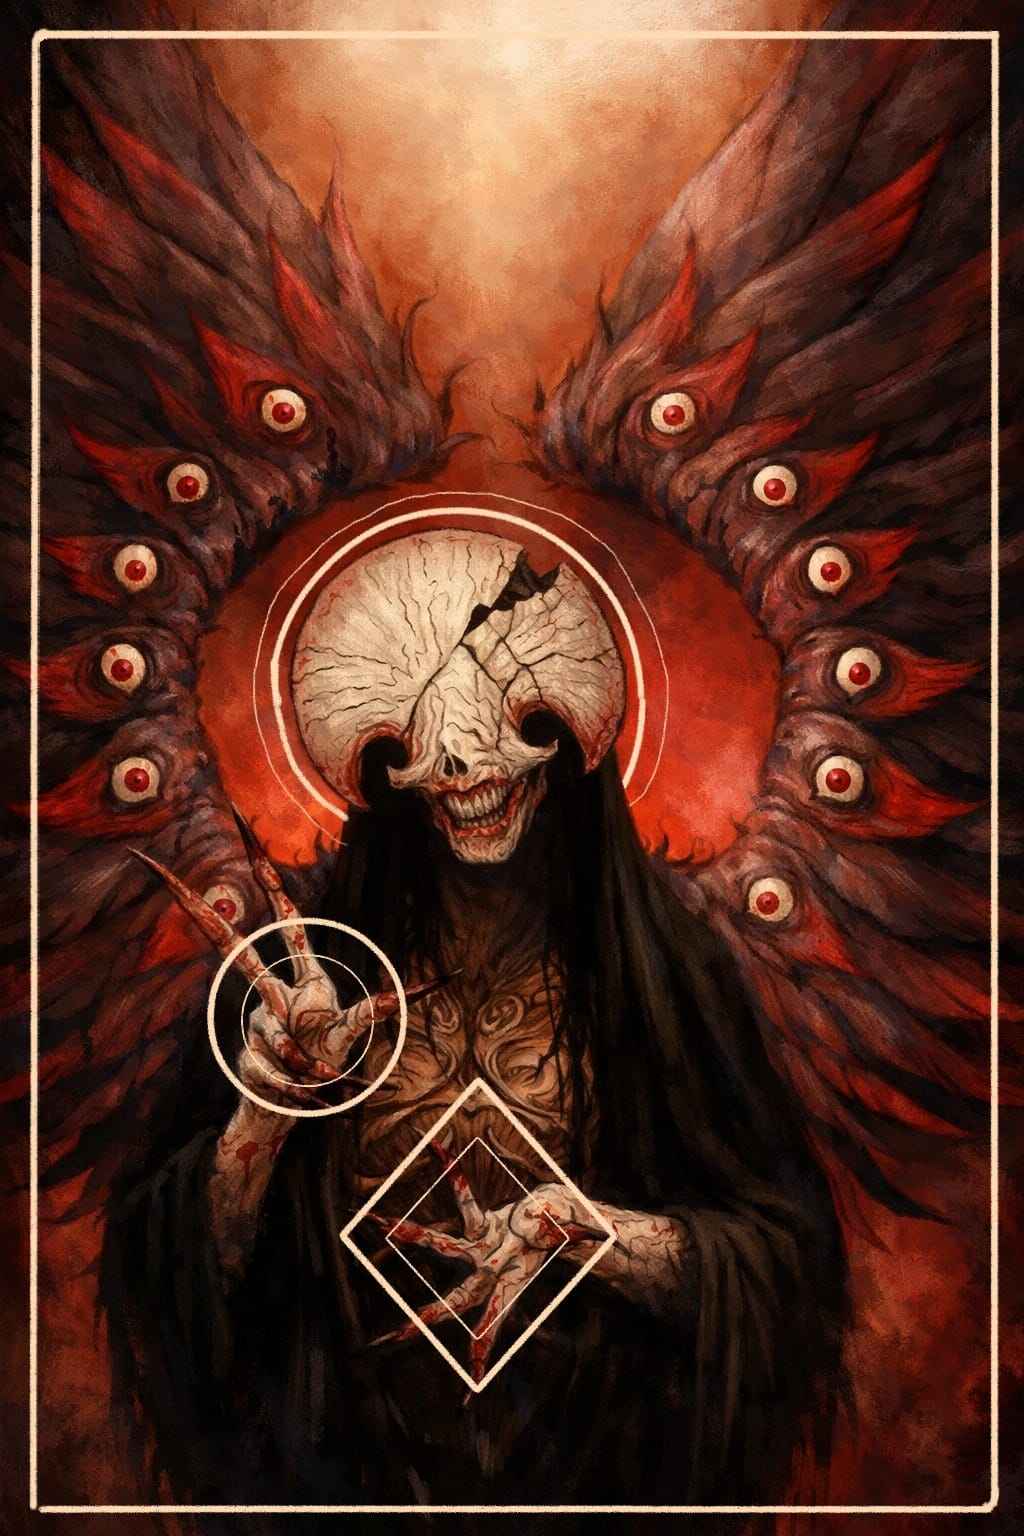
\includegraphics[width=0.75\linewidth]{Images/rotten_one.jpeg}
    \label{fig:placeholder}
\end{figure}

\subsection{}
%
%Neutral Good

\subsection{Proditism}
%Dread Wolf, orcs.
%Neutral Evil

\begin{figure}[H]
    \centering
    
\includegraphics[width=0.7\linewidth]{Images/wolf.jpeg}
    \label{fig:placeholder}
\end{figure}
